\section{Preliminaries and State of the Art}\label{sec::relwork} %Analysis \& visualization of differences in tree-structured data}\label{sec::hierarchicaldata}

\subsection{Introduction}
Today's storage capabilities facilitate the storage of a constantly growing amount of data which is most often collected and stored without filtering or preprocessing.
One of the consequences is the information overload problem defined as:

\begin{itemize}
\item Irrelevant to the current task at hand.
\item Processed or presented in an inappropriate way.
\end{itemize}

To turn these issues into advantages the science called "Visual Analytics" recently became popular. 

James J. Thomas and Kristin A. Cook coined the term "Visual Analytics"\cite{VISUAL_ANALYTICS} and defined it as: "Visual analytics is the science of analytical reasoning facilitated by interactive visual interfaces." It combines (semi-)automatic analytical analysis with interactive visualization techniques, thus emphasizes both cognitive human and electronic data processing strengths.

Whereas the information seeking mantra is described as "overview first, zoom/filter, details on demand" Keim et al define the Visual Analytics mantra as:

"Analyse First -
Show the Important -
Zoom, Filter and Analyse Further -
Details on Demand"\cite{keim2008visual}

This implies and confirms the important role of humans in the analysis process. As mentioned in the introduction humans are trained to interpret visual impressions but often fail in the same way to construe inappropriate representations (Anscombe's quartet is a very good example).

Our Visual Analytics pipeline is largely influenced by the proposal of Keim et al. (depicted in Fig. \ref{fig:visualanalyticsprocess}).

\begin{figure}[htb]
\center{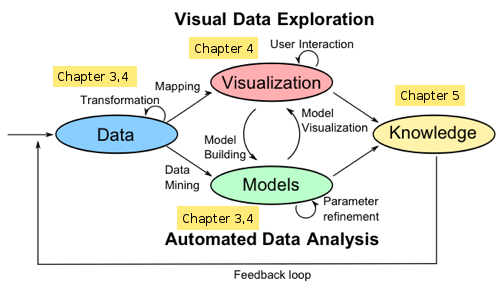
\includegraphics[width=\textwidth - 14em]
{figures/visualanalyticsprocess}}
\caption{\label{fig:visualanalyticsprocess} Visual Analytics Process proposed by Keim et al. Presented in \cite{keim2008visual}.}
\end{figure}

%Chapter \ref{sec::differences} describes the addition of new edit-operations in Treetank and two types of diff-algorithms. These fundamental to analytical reasoning and therefore denote Data Mining methods in Fig. \ref{fig:visualanalyticsprocess}. Models underlying the different views are built based on the output of the the difference-algorithms and thus represent directly the model entity in Fig. \ref{fig:visualanalyticsprocess}. Visualizations (Chapter \ref{sec::visualizations} receive user input and build models through invocation of an ID-based diff algorithm. Parameter changes in the GUI of our main visualization, a Sunburst view tailored to tree-structure comparisons, influence and change the models and in turn change the visualizations according to their output. However user interaction t havet change visualization(s) without having any impact on the model(s).

Comparing tree-structures by a Visual Analytics approach requires analytical reasoning through the computation of differences in the first place. In order to support large tree-structures we decided to use a tree-based storage system which is capable of storing transaction-time snapshots efficiently.

\subsection{Storage backend}
Treetank\cite{TREETANK} is an effective and efficient secure storage system tailored to temporal tree-structures. Currently it supports the import of XML documents which is commonly referred to as \emph{shredding}. To process stored data the W3C recommendations XPath 2.0, XQuery 1.0 and XSLT 2.0\footnote{parts of the XPath 2.0 recommendation have been implemented. Alternatively the Saxon binding can be used which also offers XPath 2.0, XQuery 1.0 and XSLT 2.0 support}, as well as a cursor like Java-API using transactions is supported. Treetank offers a pointer-based encoding and a transaction-based API to navigate in the tree-structure or modify nodes similar to the Document Object Model (DOM\cite{DOM}).

The architecture is based on three exchangeable vertical aligned layers, a transaction-layer, a node-layer and an I/O-layer. It supports \emph{Snapshot-Isolation} through Multiversion Concurrency Control (MVCC) and thus multiple readers in parallel to currently at most one writer. Furthermore the well known ACID properties are supported (Appendix \ref{subsec::acid}). Several consistency checks as of now guarantee well formed XML during serialization. While importing large XMark-instances \cite{XMark} which are commonly used for benchmarking we encountered a space-overhead due to our pointer based encoding. Appendix \ref{subsec::storage} details a number of persistent storage enhancements.

One of the most interesting properties of Treetank for our purpose is \emph{versioning}, that is storing and managing snapshots of tree-structures. Furthermore we utilize hashes which are generated for all nodes during database/resource generation, unique node-IDs as well as query-capabilities. However, Treetank does not provide any information about the changes of a node. The versioning algorithms merge \emph{NodePage}s, with the same unique ID together and override existing nodes with the latest version. NodePages organize a specified number of nodes in memory. Deleted nodes are introduced to guarantee the correctness after the merge-phase. The combination of NodePages relies on the specific revisioning algorithm. Thus, the merge-phase of NodePages usually refers to the latest full dump of all NodePages or the previous revision. As a direct consequence we are not able to simply utilize the page-layer. However a recent introduction of hook-mechanisms facilitates the indexing of changes to support comparing subsequent revisions (however, not yet implemented). Yet, such an index is only useful for comparing consecutive revisions.

The next section describes a few preliminaries for comparing tree-structures.

\subsection{Analysis of differences}
Line by line textual diffs are based on algorithms which solve the Longest Common Subsequence (LCS) problem. Whereas they are sufficient to track changes in flat text-files, tree-structures need more sophisticated methods as pointed out in the introduction.

The \emph{Extendable Markup Language} (XML) is a textual data format for encoding and structuring documents in machine- and human-readable form. Its inherent data structure is a rooted, ordered, labeled tree. 

\begin{mydef}
A rooted \textbf{tree-structure} is an acyclic connected graph, which starts with a root-node whereas every node has zero or more children and one parent-node with the exception of the root-node. We define a tree $T$ as $T = (N, E, root(T))$ whereas $N$ denotes all nodes, $E$ denotes edges, the relation between child- and parent-nodes and $root(T)$ is the root-node.
\end{mydef}

\begin{mydef}
A rooted, ordered, labeled tree is a tree-structure which extends the rooted tree-definition by defining a specific order for child nodes (that is extending the parent/child edge relation E). Furthermore each node has a label. Thus, $T$ is an ordered, labeled tree, iff $T = (N, E, root(T), \Lambda(n) \in \Sigma)$. $\Sigma$ is a finite alphabet and $n$ is a node in the tree.
\end{mydef}

Thus a tree is more restricted than a hierarchy based on a directed acyclic graph (DAG) in which every node except the root\footnote{which has no parent} has one or more parent nodes.

Many algorithms have been developed to determine differences in tree-structures for instance to provide deltas, which represent a compact version of the changes to the original document.

Next, some essential terms are defined to set the stage for the upcoming sections.

The tree-to-tree correction problem is to determine a (minimal) sequence or set of edit-operations to transform a source tree into a destination tree. 

\begin{mydef}
An edit-operation is an atomar operation which changes a tree.
\end{mydef}

A delta/edit-script is defined as:

\begin{mydef}
A delta/edit-script is a sequence or set of (elementary) edit-operations which when applied to one version v1, yields another version v2.
\end{mydef}

\begin{mydef}
A symmetric delta is a directed delta which is invertible.
\end{mydef}

In the following we use the term \emph{delta} and \emph{edit-script} interchangeably in the generic form meaning directed delta. Each edit operation is usually defined with a fixed cost (usually unit cost).

\begin{mydef}
A minimal edit script is a minimum cost edit script.
\end{mydef}

Besides providing a minimal or close to minimal edit script further metrics of a diff-algorithm are the CPU runtime and the compactness of the delta in terms of storage-space (e.g. it is in most cases sufficient to define edit operations on subtrees, such as a delete- and move-operation which usually removes respectively moves the whole subtree).

Some of the most popular approaches to detect differences in XML-documents which do not require unique node-identifiers (node-IDs) are described next.

\subsubsection{DocTreeDiff\cite{ronnau2009efficient}}
is designed for difference detection in document-centric XML documents. The algorithm computes the Longest Common Subsequence (LCS) on leaf-nodes which are on the same level by comparing hash-values. Subsequently ancestor nodes which differ are updated. Then inserted and deleted nodes are determined based on unmatched leaf-nodes in the respective tree. As only leaf-nodes which are on the same level (number of nodes on the path up to the root node) in the first step are matching candidates, the algorithm does not match identical subtrees if an inner node is added (or a leaf-node is inserted and a subtree is moved and appended to the new node which is sufficient for a tree model which only allows insertions on leaf-nodes). Furthermore moves are detected in a post-processing step instead of on the fly, thus requiring the temporary in-memory storage of inserted and deleted nodes. The runtime complexity is $O(leaves(T)D + n)$ whereas $T$ is the sum of nodes in both trees and $D$ is the number of edit operations and $n$ is the number of non-leaf-nodes. The space complexity is $O(T+D)$.%XML documents come in two-flavors. Document-centric XML documents are usually written by an author representing the structure of texts such as website-content or DocBook\cite{DocBook}-based articles whereas data-centric documents are usually automatically created through gathering data. leaf-nodes in document-centric XML usually can be discriminated very well.

%It is stated that document-centric XML typically is restricted in depth by a document format through a Schema or DTD but the width, which grows with increasing text length, is not. Furthermore almost all content is stored in the leaves whereas internal nodes represent the structure of the document (sections, paragraphs, lists, descriptions...). Based on this observation R\"onnau et al. state the following assumptions

%\begin{enumerate}
%\item Content is stored within the leaves.
%\item Changes to structure and markup will be performed on a higher level within the tree.
%\item Many non-leaf-nodes are equal due to identical markup.
%\end{enumerate}

%Based on these assumptions the algorithm relies heavily on the computation of a LCS on leaf-nodes.

%\begin{enumerate}
%\item First the algorithm computes the LCS on leaf-nodes based on their hash values and the depth in the tree.
%\item Next, a bottom up traversal of all leaf-nodes which are considered equal follows to detect updates for each anchestor node. All nodes are marked which have been processed to skip the process for subsequent bottom-up traversals when an anchestor node is the same.
%\item Last, deletes, inserts and moves are detected. A second bottom up traversal starting at leaf-nodes which have not matched, detects nodes which are in the old revision but not in the new are considered as being deleted. At every level the child nodes of the parents are searched for the nearest node which has been marked as matched during the LCS computation. If one is found the traversal stops. The same holds for inserted nodes if the reverse condition is true. Therefore the bottom-up traversal detects the largest possible subtrees to delete or insert, since the edit operations are not defined on single nodes. Furthermore adjacent deletions or insertions are glued together. Delete/insert-operations on the same subtrees are combined into one move-Operation.
%\end{enumerate}

\subsubsection{DeltaXML\cite{DELTAXML}}
Nodes are matched according to their type, the level in the tree and the Longest Common Subsequence (LCS). Furthermore matching PCDATA nodes are optionally preferred. Similar, attribute-IDs in the deltaxml-namespace may be used to mark nodes with unique IDs. Marking all nodes with an ID generates a minimum edit script. However, a complete description of the algorithm is not published.

\subsubsection{XyDiff\cite{cobena2002detecting}}
Cobena et al. present in \cite{cobena2002detecting} a fast heuristic algorithm in the context of Xyleme, an XML database warehouse. %Initially a unique persistent identifier XID is assigned to each node. XID-Maps are generated through a postorder traversal whereas initially integers from 1 to n are assigned. N denotes the number of nodes in the original tree. Added nodes in the revision to compare are assigned further integers starting from n + 1 again by a postorder traversal. Nodes which are not present in the new revision are removed resulting in gaps. Assuming an initial range of identifiers from (1-474) it might result in several ranges, for instance (1-13),(17-447),(450-474) which means that the nodes with the XIDs 14, 15 and 16 have been deleted as well as the nodes 448 and 449. The algorithm for the actual change detection is outlined in the next paragraph. Inserts, Deletes, Updates and Moves are supported. 
Signatures which are hash-values computed based on the value of the current node and all child signatures are used. Inserts and deletes are restricted to leaf-nodes in the spirit of Selkow's tree-model \cite{tai1979tree}. Based on heuristics large subtrees are matched and depending on weights propagated to parent/ancestor nodes. In \cite{ronnau2009efficient} several deltas are examined whereas the greedy subtree-algorithm yields large deltas. However, tuning parameters as the weights and how far to go up to match parent nodes is not considered.

%First nodes with ID attributes defined in a DTD are matched. Then signatures are generated in a bottom-up traversal, which are hash values computed from the value of the current node and all child signatures. Furthermore weights are computed and defined as the text node sizes which are summed up for each child node. A priority queue is build, whereas the largest weights of the new document are prioritised. The largest subtrees are considered first to be matched based on their signatures. If more than one node has the same signature a heuristic is used, otherwise the child nodes are added to the queue. Whenever nodes match each subtree and anchestor pair is going to be matched as long as the labels are equal. The propagation to anchestor nodes depends on the node weight. A heuristic is used to substitute the computation of largest order preserving common subsequences for the move-operation. As heuristics are used the resulting edit-scripts/deltas are not guaranteed to be minimal.

The CPU runtime of the algorithm is $O(n \log n)$ and the space complexity is $O(n)$ whereas $n$ is the size of both documents.

\subsubsection{LaDiff / Fast Match Simple Editscript (FMSE)\cite{chawathe1996change}}\label{subsec::ladiff}
operates on different versions of LaTeX documents. We describe the algorithm in slightly more detail as we decided to implement the algorithm for XML data in Treetank. It is developed in the context of \LaTeX to demonstrate and measure the feasibility of an approach to detect changes in hierarchically structured information. 

Chawathe et al. divides this task into two main problems:

\begin{description}
\item[the Good Matching problem] is the problem of finding matches between the two trees, which are either equal for some predefined function or approximately equal.
\item[finding a Minimum Conforming Edit Script (MCES)] is the second obstacle. Recapitulate that an \emph{edit script} is a sequence of edit operations transforming the source file into the target document once applied. Costs are therefore applied to every edit operation.
\end{description}

The algorithms used to solve these two problems operate on rooted, ordered, labeled trees. Four edit operations (\texttt{insert}, \texttt{delete}, \texttt{update} and \texttt{move}) are defined with unit costs such that an \texttt{insert}/\texttt{delete} or \texttt{delete}/\texttt{insert} is more costly than a \texttt{move}.

The algorithm proves to yield minimum edit scripts in case the assumption holds true that no more than one leaf-node is considered equal to a predefined function which compares the values of leaf-nodes and the labels match. XML does provide labels in form of \texttt{QName}s for \texttt{element}- and \texttt{attribute}-nodes (as well as attribute-values) and a slightly restricted alphabet for \texttt{text}-nodes. Thus either text-node values have to be compared, \texttt{QName}s or \texttt{QName}s and attribute-values.

The first criterion defined for leaf-nodes is 

\begin{equation} 
compare(v(x), v(y)) \leq f\ such\ that\ 0 \leq f \leq 1
\end{equation}

Inner nodes are matching candidates according to

\begin{equation}
\frac{|common(x, y)|}{max(|x|,|y|)} > t\ and\ label(x) = label(y)
\end{equation}

\begin{equation}
common(x,y) = \{(w,z) \in M | x\ contains\ w\ and\ y\ contains\ z\}
\end{equation}

whereas a ``node x contains a node y, iff y is a leaf-node descendant of x and $|x|$ denotes the number of leaf-nodes x contains''. The threshold t is defined as $0.5 \leq t \leq 1.0$.

In a first step the good matching problem is solved by means of concatenating nodes/labels bottom up during a postorder traversal and finding a longest common subsequence (LCS). Furthermore, nodes which are unmatched during the LCS-matching are subject to a subsequent comparison. The predefined similarity-function is applied and if the nodes are matched they must be aligned. 

After that in a breadth first traversal nodes are inserted, updated or moved. The children of each node are aligned based on the LCS once again. Nodes which are matched but not in the LCS are moved. The order in which operations are applied to the source tree and the edit script is crucial to the correctness of the algorithm. Details are omitted for brevity.

The second step is the deletion of unmatched nodes during a postorder-traversal.

When the assumption which assures the generation of a minimum edit-script does not hold which might be the case for several XML-documents, especially in data centric XML files, the algorithm yields large output-deltas due to mismatches according to Lindholm et al.\cite{lindholm2006fast} and Rönnau et al.\cite{ronnau2009efficient}. This is a direct consequence of the ambiguity of the LCS as well as of the subsequent matching of nodes. However this is a problem common to almost all differencing algorithms and can be minimized by proper definitions of the similarity functions for leaf- and inner-nodes. An optional post-processing step reduces mismatches and thus move-operations such that children of matched nodes, which do not have same parent are candidates for matches with children of the same parent in the other tree, thus correcting some misaligned nodes. Note that this step can not reduce errors, which are propagated from mismatched leaf-nodes.

It becomes apparent by investigating the analysis of Rönnau et al.\cite{ronnau2009efficient} that the result of mismatched leaf-nodes in contrast to other algorithms yields many moves (compared to more inserts/deletes in other algorithms). However, moves in Treetank without generating hashes and storing the number of descendants of each node during import are a constant time ($O(1)$) operation due to the pointer-based approach. Even with hashing enabled which provides inevitable performance-boosts for our internal ID-based diffing algorithm which is used in a subsequent step by our visualizations, only ancestor nodes are affected and thus linear time is needed (however much faster than a deletion and insertion which in addition requires traversing the whole subtree two times).

The runtime complexity is $O(n \cdot e + e^2)$ and the space complexity is $O(n)$ whereas $n$ is the number of unchanged nodes and $e$ is the number of different/changed nodes.

\subsubsection{X-Diff\cite{wang2003x}}
operates on unordered, labeled trees. Thus the order of child nodes does not matter. Despite using an unordered tree-model which is not suitable in many cases as for instance document centric XML, updates on element nodes to the best of our knowledge are not defined as the signature for \texttt{TextNode}s does not use their values. However updating an internal node is crucial due to otherwise potentially large subtree delete- and insert-operations even though only a single node is updated.

%First XHash values are computed in a bottom up postorder traversal for every node which represent the entire subtree rooted at the respective node.
%The hash computation does not include the child order, such that isomporhic trees can be matched in subsequent steps.

%Next the trees are traversed starting from the root-nodes. Nodes on currentLevel+1 are filtered out which have equal hash values.

%Signatures defined as $Signature(x) = /name(x_{1})/.../name(x_{n})/name(x)/type(x)$ for element nodes and $Signature(x) = /name(x_{1})/.../name(x_{n})/type(x)$ for text nodes are used to determine if nodes are considered to match. Note that in case of a text node it does not contain the value in the signature. This decision leads to the support of update-Operations, which are only defined as an edit cost for text nodes. 

%Initially leaf-nodes are compared based on a predefined edit distance function and a matching/distance-value tuple is stored in a table. To compute the edit distance between subtrees the minimum-cost maximum flow algorithm \cite{zhang1996constrained} is used.

%Based on a minimum cost matching and the distance table an edit script can be computed.

The runtime is defined for three involved steps separately: 

\begin{enumerate}
\item {\bf{Parsing and Hashing}}: $O(|T_{1}| + |T_{2}|)$
\item {\bf{Mapping}}: $O(|T_{1}| \times |T_{2}|) \times max\{deg(T_{1}, deg(T_{2})\} \times \log_{2}(max\{deg(T_{1}), deg(T_{2})\}))$
\item {\bf{Generating Minimum-Cost Edit Script}}: $O(|T_{1}| + |T_{2}|)$
\end{enumerate}

\subsubsection{Faxma\cite{lindholm2006fast}}
uses fast sequence aligning transforming the parsed documents into sequences of tokens. Subsequently the diff is computed using rolling-hashes with different window-sizes. Moves are handled through the combination of \texttt{delete/insert} pairs which is similar to the approach used by \emph{DocTreeDiff}. The delta is a script which includes identifiers to matched nodes with inserted sequences in between. It is thus not defined in terms of a usual edit script and therefore not directly useful for our purpose.   %First the input documents are parsed into XAS tokens, which preserves the XML structure. They support three edit operations: \texttt{insert}, \texttt{delete} and \texttt{move} since they claim that subtrees are often moved. . Based on \emph{rolling-hashes} a sliding window iterates over sequences derived from transforming both XML documents. A rolling-hash can be updated really fast if the right hash-function is chosen. If so, only the old value, the new value and the previous hash-value is needed \cite{RollingHash}:

%\begin{equation}
%h(S_{i+1}) = H(h(S_{i}), s_{i} , s_{i+n+1})
%\end{equation}

%To quickly find maximum length matches, window sizes of length $S = <48,32,16,8,4,2,1>$ are used.

%At first all nodes are marked as $ins(node)$ in both sequences. Starting with the greatest size, matches are searched for in a zigzag-pattern, whereas matched sequences are extended alternately moving forward and backward until no further matches are found. These matches are marked with\\ $cpy([start\ index], [end\ index])$ in the sequence of the updated document. Any matching sequences are then removed from the sequence representing the old revision, finally resulting in the configuration, that only deleted nodes are left in this sequence.

%Since the matches are not necessarily aligned on subtree boundaries the match-list must be transformed back into the tree-domain.

%The algorithm serializes match lists in a sequential traversal, providing the \texttt{start-} and \texttt{end-tag} has been encountered. A queue of tentative node- and tree-reference tags is maintained to either discard changes partially or serialize the results. Details of this algorithm are omitted, since the resulting delta does not fit our purpose. The delta is a script which includes identifiers to matched nodes with inserted sequences between. It is thus not defined in terms of an edit script and thus not directly useful for our purpose.

\subsubsection{Summary}
The problem in common to all approaches is to efficiently compute a minimum or near minimum edit script in order to transform the first into the second tree. Unfortunately a guaranteed minimum edit script for the the tree-to-tree correction problem is known to be bound in runtime by \\$O(nm\ min(depth(T1),\ leaves(T1))\ min(depth(T2),\ leaves(T2)))$, with $n$, $m$ denoting the number of nodes of the trees $T1$ , $T2$\cite{Zhang:1989:SFA:76071.76082}. Using heuristics speeds up the process but in most cases generates non optimal (non minimal) edit scripts. These non minimal deltas are counterintuitive when used to determine differences between tree-structures, because of mismatched nodes. These mismatches result in modifications of nodes which should not be changed and vice versa. However detecting changes is not our primary obstacle, which requires monitoring. Even algorithms which guarantee a minimum edit script do not necessarily reflect the changes due to their inherent ambiguity. Usually a few edit-scripts are minimal according to their cost-model of edit-operations.

Every diff-algorithm has its strength and pitfalls. Depending on the input and expected modification patterns some algorithms provide better results than others in terms of predefined evaluation criteria. Even though several algorithms are compared in \cite{ronnau2009efficient} we remain critical as the size of the delta and the amount of edit-operations might not be the best discriminator. The granularity and the cost of edit-operations is equally important. For instance the cost of the moves in Treetank at worst is linear in the number of ancestor nodes, the sum of ancestors of the node before it is moved and afterwards and constant at best, depending on configuration options\footnote{generating hashes and determining the number of descendants of each node or not}. Defining insertions and deletions in terms of subtrees reduces the size of the edit-script. However it does not take the cost of applying these changes into account. That said all algorithms work best if leaf-nodes are distinguishable very well and thus the similarity measures are able to match only one node in the other tree. Otherwise finding a best match for each node results in at least a quadratic runtime. Comparing document oriented XML thus usually produces better results in comparison to data centric XML in terms of minimum or near minimum edit-scripts/deltas.

Memory consumption is very important considering large XML instances ranging from 10 MiB to 100 MiB and more. However at some point either the trees have to be splitted or costly I/O operations due to serialization/deserialization of data structures on external storage have to be used. Reducing the cost of computing the LCS which has a large memory footprint might be mandatory but also results in heuristics. A survey of the wide range of algorithms is summarized in \cite{cobena2002comparative}. Several algorithms are described and compared according to the attributes memory consumption, time complexity, supported operations and the tree model. However it does not include comparisons of recent algorithms as DocTreeDiff and Faxma. Thus, a short summary is detailed in Table \ref{chap2:Comparison}. DeltaXML 

In summary a trade-off between the number of edit-operations, the memory consumption and the runtime complexity of the algorithm exists. Furthermore no algorithm exists which outperforms and in respect to the edit-script cost produces always better results than the others while comparing trees of different domains and characteristics. It heavily depends on the change pattern of the input document and parameters of the algorithm if provided. Due to the different granularity of the edit-operations among the approaches the size of the delta and the number of different types of edit-operations is not always a good evaluation criteria. To be fair the cost of applying all edit-operations must be determined. Thus, the cost of insertions and deletions is always defined on the subtree-sizes.

\begin{table}[tb]
\begin{minipage}{\linewidth}
\centering 
\begin{tabularx}{0.9\textwidth}{|l|>{\centering\arraybackslash}X|>{\centering\arraybackslash}X|>{\centering\arraybackslash}X|>{\centering\arraybackslash}X|>{\centering\arraybackslash}X|>{\centering\arraybackslash}X|>{\centering\arraybackslash}X|} 
\hline
\textbf{algorithm} & \textbf{runtime} & \textbf{space} & \textbf{tree model} & \textbf{move support}\\
\hline
\hline
\textbf{DeltaXML} & not published & not published & not published & not published\\
\hline
\textbf{XyDiff} & $O(n \log n)$ & $O(n)$ & ordered & yes\\
\hline
\textbf{FMSE} & $O(n \cdot e + e^2)$ & $O(n)$ & ordered & yes\\
\hline
\textbf{X-Diff} & $O(n^2)$ & not published & unordered & no\\
\hline
\textbf{DocTreeDiff} & $O(leaves(T)D + n)$ & $O(T+D)$ & ordered & yes\\
\hline
\textbf{Faxma} & $O(n)$ (average) & not published & ordered & no\\
& $O(n^2)$ (worst) &  & & \\
\hline
\end{tabularx}
\label{chap2:Comparison}
\vspace{0.5em} 
\caption{Comparison of tree-to-tree difference algorithms.}
\end{minipage}
\end{table}

\subsection{Visualization of differences}
In the past several visualization techniques have been proposed for hierarchical data ranging from simple node link diagrams, force directed layouts to space filling approaches. Comparison of tree-structures just recently gained momentum. %Recently database systems which are capable of storing hierarchical temporal data efficiently and therefore store snapshots of time varying data put forth the need to analyse these data. %to determine and visualize changes between several revisions such that analysts are able to answer time dependent questions like the ones raised in the motivating application examples.

%While in the past it has been possible to map temporal hierarchical data to relational databases it required the storage of a full snapshot through foreign/primary key relations instead of just storing incremental or differential updates as well as the hierarchical mapping overhead.

%\subsubsection{TimeRadarTrees\cite{vilanovatimeradartrees}} To visualize weighted dynamic compound Digraphs, which are graphs with a hierarchical dimension, TimeRadarTrees have been developed. Changes of leaf-nodes and their directed edges are revealed, whereas incoming edges are plotted in a radial manner as a slice on the inner circle. Outgoing edges are represented by the outer thumbnails. Therefore visual clutter regarding related nodes, which occurs in node link diagrams is avoided. The hierarchy and thus the inner nodes are drawn on top of the inner radial circle (Fig. \ref{fig:timeradar}). The leaf-nodes are labeled A, B, C, D and E. Each segment of a node represents the node in a specific revision of the graph. Node D has three incoming edges in the first graph, in the second one and in the third none (inner circle). The color red denotes that the node has at least one incoming or outgoing (which depends on whether one looks at the inner or outer circles) edge. Grey scale means the node has no incoming/outgoing edges at all. As TimeRadarTrees visualize changes on leaf-nodes but not the hierarchy itself they can not be directly mapped to our task and thus are not present in the short evaluation at the end of this chapter and in table \ref{chap2:Comparison}.

%\begin{figure}[tb]
%\center{\includegraphics[width=\textwidth - 12.5em]
%{figures/timeradar}}Phylogenetic trees among a nontrivial number of input sequences are constructed using computational phylogenetic methods. Distance-matrix methods such as neighbor-joining or UPGMA, which calculate genetic distance from multiple sequence alignments, are simplest to implement, but do not invoke an evolutionary model. Many sequence alignment methods such as ClustalW also create trees by using the simpler algorithms (i.e. those based on distance) of tree construction. Maximum parsimony is another simple method of estimating phylogenetic trees, but implies an implicit model of evolution (i.e. parsimony). More advanced methods use the optimality criterion of maximum likelihood, often within a Bayesian Framework, and apply an explicit model of evolution to phylogenetic tree estimation.[3] Identifying the optimal tree using many of these techniques is NP-hard,[3] so heuristic search and optimization methods are used in combination with tree-scoring functions to identify a reasonably good tree that fits the data.
%Tree-building methods can be assessed on the basis of several criteria:[6]
%\caption{\label{fig:timeradar} TimeRadarTrees illustration. Presented in \cite{vilanovatimeradartrees}.}
%\end{figure}

\subsubsection{Treevolution\cite{theron2006hierarchical}} visualizes the evolution of hierarchical data in a radial node-link diagram. Each node might have arbitrary many parent nodes and each ring represents one snapshot of the hierarchy. Inserted nodes are placed on the appropriate ring depending on the time of insertion. However edge crossings occur frequently due to the parent-child relationship whereas often times nodes have more than one parent. A direct consequence is visual clutter which complicates the analysis of the hierarchical relationship between inserted nodes and their parents. Furthermore label overplotting occurs frequently which is a result from drawing the labels in one direction (left to right), however a simple interaction method improves on this by providing rotation mechanisms.

\subsubsection{Interactive Visual Comparison of Multiple Trees\cite{bremm2011interactive}} The authors propose a prototype to compare multiple phylogenetic trees. Several views are available to analyse the trees on different levels of detail. A matrix view for instance displays pairwise tree-similarities based on a similarity score which takes overlapping subtrees into account. The similarity score depends on all nodes in a subtree including inner nodes instead of just determining overlapping leaf-nodes. A histogram shows the score distribution among all nodes in all trees. The consensus tree is "a compact form of representing an 1:n comparison" in one tree. The score is "the average of the scores comparing a reference tree node against its best matching unit in all other trees". The last view is a Tree Comparison View which highlights all nodes in the subtree a user marks through a linking and brushing technique in all other trees. It is the only system which is capable of comparing multiple trees on different levels of detail at the same time with linked visualizations. However we assume that the quadratic runtime of comparing all nodes with all other nodes will be restricted to (many) small trees. Furthermore to the best of our knowledge it is not mentioned how nodes are compared, but we assume unique labels or node identifiers are required as the prototype is proposed for phylogenetic trees. 

\subsubsection{Spiral-Treemap/Contrast-Treemap\cite{tu2007visualizing}}
A Treemap is a space filling approach which maximizes available screen space for the visualization. Most treemap layouts suffer from abrupt significant layout changes even if the underlying data changes were rather small. Tu et al. propose a new layout algorithm called \emph{Spiral Treemap} to improve the layout stability arranging child nodes in spirals which change the orientation by 90° in the corners. Child-nodes are aligned along a spiral in each level beginning at the upper left corner. Therefore edit-operations as for instance \texttt{inserts} and \texttt{deletes} only affect local regions. However, we argue that it is not trivial to analyse structural differences as they are not explicitly visualized in the Contrast Treemap and the texture distortion depends on the layout algorithm, whereas small changes are hardly visible. Furthermore the hierarchy is not easy to recognize in the Spiral Treemap which is a common problem for Treemaps owed to the enclosing nature of child nodes in their parent nodes. Labels however are easily perceived if the rectangles are not too thin which occurs frequently in large trees ranging from about $50000$ nodes to a few hundred or even millions of nodes. Furthermore the nodes degenerate from rectangles to very tiny stripes. Improving the aspect ratio of the rectangles results in Squarified Treemaps\cite{bruls2000squarified}, which lack the property of ordered siblings. However child-nodes in trees are often ordered which is why Squarified Treemaps in general are only feasible in certain specific cases which lack a semantic difference in node ordering. %(Fig. \ref{fig:treemap-spiral}). Furthermore \emph{Contrast Treemaps} are proposed to visualize attribute changes. First a union tree is build to merge the two trees. Inserted and Deleted nodes are missing the corresponding attribute value in the other tree. Otherwise two attribute values are available from each tree, which are color coded in the same rectangle. The value of the "original" item is in the top left corner whereas the other value is in the bottom-right. Additionally it is possible to encode the value depending on the occupied area. The higher the value in one tree the more area is occupied, the lower the value the fewer area is utilized. The Spiral Treemap layout algorithm is used whereas the size of the items in the Treemap is based on one of the attribute values or an aggregation function (min, max, avg). Another technique helps tracking layout changes. A background image is placed behind one of the two Treemaps representing one of the trees. It is distorted in regions which have changed due to the second Treemap layout. Regions which are extended or shrinked are also reflected in the distortion of the background image. Note, that in order to gain knowledge from the distorted texture/image a stable layout algorithm as for instance the Slice and Dice or Spiral Treemap is required. 

%\begin{figure}[tb]
%\center{\includegraphics[width=\textwidth]
%{figures/treemap-spiral}}
%\caption{\label{fig:treemap-spiral} Spiral Treemap. Presented in \cite{tu2007visualizing}.}
%\end{figure}



%\begin{figure}[tb]
%\center{\includegraphics[width=\textwidth]
%{figures/treevolution}}
%\caption{\label{fig:treevolution} Treevolution. Presented in \cite{theron2006hierarchical}.}
%\end{figure}

\subsubsection{TreeJuxtaposer\cite{munzner2003treejuxtaposer}}
TreeJuxtaposer is a system designed to support biologists to compare the structures of phylogenetic trees. A new Comparison algorithm to determine matching nodes in near-linear average time is proposed. Perfect matching nodes have the same labels for each of their leaf-nodes. Based on a simple similarity measure ($S(A,B)$ between two sets whereas the function is defined as $\frac{A \cup B}{A \cap B}$) they propose a method to colorize edges of non perfectly matching nodes and a rectangular magnifier to emphasize changed nodes. The visualization itself contains several revisions side by side plotted in node-link diagrams. Selections and rectangular magnifications are synchronized. TreeJuxtaposer uses a node-link algorithm and thus shares the drawbacks of other node-link visualizations such as \emph{Treevolution} and the \emph{Ripple presentation}. In comparison to space filling approaches further attributes as for instance value comparisons, subtree-sizes and labels are not visualized or result in visual clutter. Furthermore the fast differencing algorithm to the best of our knowledge relies on unique node labels to support the region query on a two-dimensional plane.

%\begin{figure}[tb]
%\center{\includegraphics[width=\textwidth]
%{figures/treejuxtaposer}}
%\caption{\label{fig:treejuxtaposer} TreeJuxtaposer. Presented in \cite{munzner2003treejuxtaposer}.}
%\end{figure}

\subsubsection{Code Flows: Visualizing Structural Evolution of Source Code\cite{telea2008code}}
Code Flows is proposed for determining and tracking changes in source code between several revisions. It is a space filling approach which uses horizontally mirrored icicles and therefore additional attributes of nodes are visualizable besides highlighting actual tree changes. Labels are readable in smaller trees or when zoomed in because of the rectangular layout of icicle plots. Due to spline-tubes matching, nodes can be tracked very well through different revisions. Even code splits and merges are easily trackable. On the downside small code changes resulting in the addition or deletion of a few nodes might not be visible at first glance. Furthermore the spline connections between matched nodes leads to visual clutter due to overplotting when nodes are moved.

%\begin{figure}[tb]
%\center{\includegraphics[width=\textwidth - 15em]
%{figures/codeflows}}
%\caption{\label{fig:codeflows} Code Flows. Presented in \cite{telea2008code}.}
%\end{figure}

\subsubsection{Ripple presentation for tree structures with historical information\cite{ishihara2006ripple}}
The Ripple presentation visualizes both evolving hierarchies and categories. Concentric circles are used to indicate an evolving hierarchy through time. Each circle represents one point in time. Nodes are plotted in a special node-link layout. The root node of each subtree is in the focus of the view. leaf-nodes are arranged in ascending order meaning older nodes are drawn on circles further away from the current root of the subtree. The angles of edges are application dependent and facilitate the clustering of categories through time. In their news articles, example categories are extractable from the content. For each child belonging to the same category the angle of the edge has to be located in between the parent angle. Since the application examples require no diff-calculation and updates as well as deletions of nodes are not considered it is not useful to compare every aspect of changing tree structures. It suffers from a lot of clutter consequent to label overplotting as well. Deletions and updates have not been considered since the example use cases to the best of our knowledge just add nodes and categories. Due to the fact that it is also a node link representation and not a space filling approach attributes of nodes are not visualizable. Thus it is best comparable to Treevolution, but because of the more complex layout algorithm it can group nodes according to categories. 

%\begin{figure}[tb]
%\center{\includegraphics[width=\textwidth - 12em]
%{figures/ripple}}
%\caption{\label{fig:ripple} Ripple presentation. Presented in \cite{ishihara2006ripple}.}
%\end{figure}

\begin{table}[tb]
\begin{minipage}{\linewidth}
\centering 
\begin{tabularx}{0.9\textwidth}{|l|>{\centering\arraybackslash}X|>{\centering\arraybackslash}X|>{\centering\arraybackslash}X|>{\centering\arraybackslash}X|>{\centering\arraybackslash}X|>{\centering\arraybackslash}X|>{\centering\arraybackslash}X|} 
\hline
\textbf{visualization} & \textbf{hierarchy} & \textbf{space filling} & \textbf{readability} & \textbf{changes}\\
\hline
%\hline
%\textbf{Sunburst} & +++ & ++ & + & +++\\
\hline
\textbf{Spiral-/Contrast-Treemap} & + & ++\footnote{due to the side by side view which needs a lot of space} & ++ & ++\\
\hline
\textbf{Treevolution} & + & - & + & +\\
\hline
\textbf{Code Flows} & +++ & ++ & ++ & ++\\
\hline
\textbf{Juxtaposer} & ++ & - & ++ & +++\\
\hline
\textbf{Ripple Presentation} & + & - & + & +\\
\hline
\textbf{IVCoMT} & +++ & - & ++ & ++ \\
\hline
\end{tabularx}
\label{chap2:Comparison}
\vspace{0.5em} 
\caption{Comparison of tree-to-tree comparison visualizations. "-" indicates the absence of an attribute, "+" to "+++" implies how well or bad the attribute is supported.}
\end{minipage}
\end{table}

\subsubsection{Summary}
Recently, interactive visualizations of the evolution of tree-structures or different, similar trees have been proposed. Table \ref{chap2:Comparison} summarizes the visualizations according to several attributes. The first column denotes the readability of the hierarchy-representation. The second column indicates if a space filling approach is used and to which extend the whole display space is utilized. The third column characterizes the readability of the visualization including the encoding of differences and labels. The last column is the most significant. It determines to which extent changes are visualized. Even deletions are not considered in some cases which might be due to the use cases of the respective visualization. Note that the scale ranges from "-", not present to "+++" (best). Chapter \ref{sec::conclusion} presents a detailed more comprehensive analysis in comparison to our system. 

Most of the visualizations are tailored to specific tasks and thus are at best only partially useful for other applications. In fact besides adapting the diff-algorithm described in \cite{telea2008code} none of the proposed systems to the best of our knowledge is able to compare every kind of tree structure due to diff-algorithms which rely on domain characteristics as unique node identifiers/node labels or on change detections which hook into a system. Furthermore we suppose that except TreeJuxtaposer and CodeFlows no other system is able to compare large trees. However, in CodeFlows the filtering of nodes depends on the level of detail (per class-level, function-level...). Thus a global view which filters all relevant, changed nodes is not available.

The prototype presented in \cite{bremm2011interactive} by Bremm et al. is the only system capable of visualizing differences at various levels of detail due to linked visualizations. However, we are observe, that the approach in its current form is not applicable to large tree-structures due to their similarity measures which pose a quadratic runtime complexity.

%The use cases of \emph{TimeRadarTrees} are rather different from the ones addressed in this thesis. While changes of leaf-nodes and the relationships between them are in the focus of TimeRadarTrees, determining and visualizing changes of the whole hierarchy is one of the main goals in this thesis.



%\emph{Ripple presentations} 

%\begin{figure}[tb]
%\center{\includegraphics[width=\textwidth - 12em]
%{figures/ripple-clutter}}
%\caption{\label{fig:ripple-clutter} Ripple representation - label overplotting. Presented in \cite{ishihara2006ripple}.}
%\end{figure}

%\emph{TreeJuxtaposer} 

%\emph{Code flows}

%\emph{Interactive Visual Comparison of Multiple Trees} 






